\documentclass[../root]{subfiles}
\graphicspath{{_images/}{../_images/}}

\begin{document}

    \chapter{Month-of-Birth Effects on Skills and Skill Formation}

    \begin{shortsummary}
        \begin{itemize}
            \item \authoryear{Yamaguchietal2020}
            \item \RQ{To what extent month of birth affects one's well-being? How children and ttheir parents respond to the shocks beyond redshirting?}
            \item \answer{Linear regression of outcomes on the relative age of the students, using longitudial data of student in public schools in Japan in 2015-'18.}
            \item \result{The gaps between the relative ages were observed in both cognitive and noncognitive skills, which also leads younger students and their parents to responding to the disadvantages.}
        \end{itemize}
    \end{shortsummary}

    \section{Introduction}

    \paragraph{Month of birth effects}

    \begin{itemize}
      \item Many papers have documented that relatively younger students suffer a disadvantage.
      \begin{itemize}
        \item Academic tests: Bedard and Dhuey (2006)
        \item Sports: Helsen et al. (2005)
        \item other school activities: Dhuey and Lipscomb (2008)
        \item Long-term outcomes: Bedard and Dhuey (2006), Kawaguchi (2011), Du et al. (2012), Muller and Page (2016).
      \end{itemize}
      \item However, less is known how children and their parents respond to the negative birth month shocks.
      \begin{itemize}
        \item Compensatory investment: time usage of study outside school.
        \item Interpersonal relationships.
      \end{itemize}
    \end{itemize}

    \paragraph{Objectives and Strategy}

    \begin{itemize}
      \item To estimate the effects of month of birth on:
      \begin{itemize}
        \item cognitive and noncognitive skills.
        \item Time use, prep school attendance, participation in sports, and the quality of relationships with teachers and peer students.
      \end{itemize}
      \item Data: longitudinal data of all fourth to ninth graders in public schools in an anonymous province in Japan in 2015-2018.
      \begin{itemize}
        \item Redshirting is virtually impossible in Japan (Similar to England, Norway, and Iceland): The month of birth is exogeneous.
      \end{itemize}
    \end{itemize}

    \paragraph{Results}

    \begin{itemize}
      \item The month of birth affects both cognitive and noncognitive skills.
      \begin{itemize}
        \item Relative age influences the formation of noncognitive skills.
      \end{itemize}
      \item Youngest students in the ninth grade work more outside of school than the oldest students.
      \begin{itemize}
        \item Also read for more hours and more likely to attend a prep school.
        \item Fewer hours on sports, arts, and music (may affect formation of noncognitive skills: Ishihara et al. (2018); Moreno et al. (2011)).
      \end{itemize}
      \item Younger students suffer interpersonal relationships.
    \end{itemize}

    \paragraph{Contribution}

    \begin{itemize}
      \item Implication for efficiency and equity.
      \begin{itemize}
        \item The existing school cutoff date may distort students' and their parents' skill investment behavior.
        \item Policies mitigating month-of birth effects could correct this distortion.
      \end{itemize}
      \item Long-term development of noncognitive skills, which might account for the lower earnings in adulthood.
      \begin{itemize}
        \item Results may explain this long-term consequences in some countries: Kawaguchi (2011).
      \end{itemize}
    \end{itemize}

    \section{Empirical Strategy}
    \subsection{Econometric Model}

    \begin{itemize}
      \item The youngest children in a given grade were born in March and the oldest in April in Japan.
      \item Estimation is made separately for each grade using the following econometric model:
      \[
      Y_{it} = \beta_0 + \beta_1 + \text{AGE}_{it} + \beta_2 \text{AGE}_{it}^2 + \beta_3 X_{it} + \epsilon_{it}.
      \]
      \begin{itemize}
        \item $Y_{it}$: an outcome for student $i$ in year $t$
        \item $\text{AGE}_{it}$: normalized relative age at test measured in months.
        \item $X_{it}$: Covariates including gender, \# of books at home as a proxy for SES, year, school ficed effects.
      \end{itemize}
      \item The estimated gap between the oldest and youngest students:
      \[
      \hat{\Delta Y} = \hat{\beta}_1 \cdot 11 + \hat{\beta}_2 \cdot 11^2
      \]
      \item Three factors generated by the relative age gap:
      \begin{enumerate}
        \item The absolute age effect.
        \item The effect of age at school entry.
        \item The effect of relative age.
      \end{enumerate}
      \item Because of the high correlation to each other, they do not attemt to identify the effect separately.
      \item Endogeneity bias: timing of birth
    \end{itemize}

    \subsection{Assesing Exogeneity of Month of Birth}

    \begin{itemize}
      \item The main limitaion is the shortage of variables about family/paretal characteristics.
      \item Two exercises to overcome the problem using: vital statistics, and administrative data.
    \end{itemize}

    \paragraph{Vital Statistics} 人口動態統計

    \begin{itemize}
      \item The adjusted birth month shares: the share is statistically significantly different from complete random, but the magnitudes are small. (Figure 1)
      \begin{figure}[ht]
        \centering
        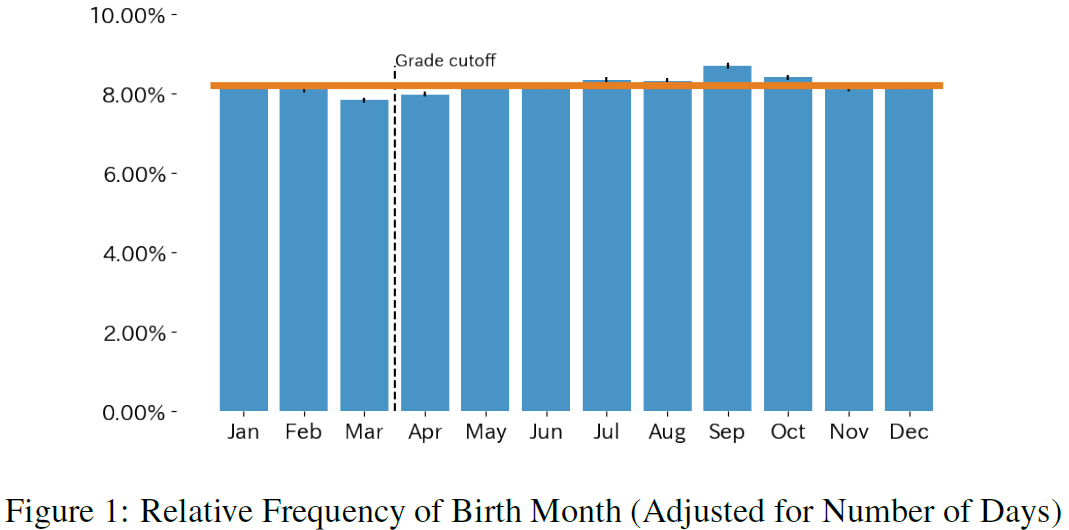
\includegraphics[scale = .6]{0904tanji/F1}
      \end{figure}
      \item Regression of parental characteristics and birth outcomes on age, agesquared, and birth-year dummies (p-values using the method proposed by Benjamini and Hochberg (1995)). (Table 2)
      \begin{itemize}
        \item Educated mothers may try to time birth so that their child is born in April: no significant gap.
        \item The occupations of household head: no significant gap except for non-regular employment.
        \item Seasonal effect on children's health: significant in that April-born children are less likely to be a first child (possible downward bias).
        \begin{itemize}
          \item Literature says that first-born children tend to perform better than their younger siblings.
        \end{itemize}
      \end{itemize}
      \begin{figure}[ht]
        \centering
        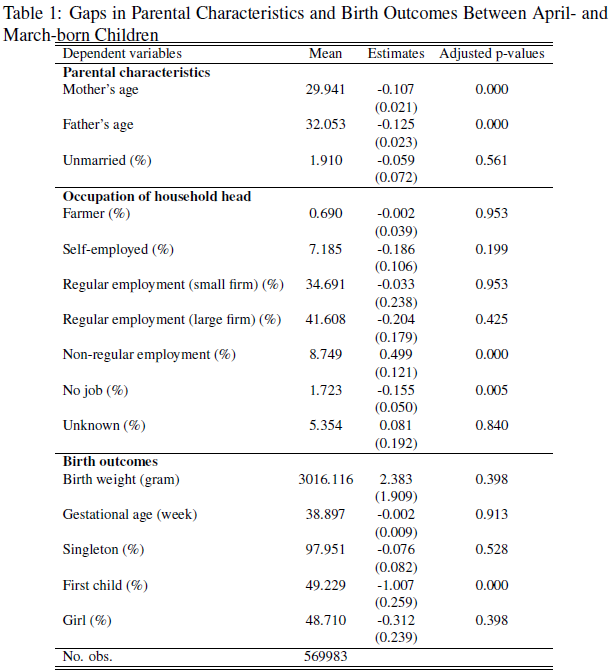
\includegraphics[scale = 1]{0904tanji/T1}
      \end{figure}
    \end{itemize}

    \paragraph{Administrative Data}from a municipality.

    \begin{itemize}
      \item include information on whether a family is on welfare, receives an education subsidy as a low-income family, and/or a single-parent household for 11,942 students in 2015 and 2018.
      \item Regrression of family SES variables (Table 2).
      \begin{itemize}
        \item No significant correlation between birth month and family SES measures.
        \item The number of books: little statistical and economic difference is seen between the two.
      \end{itemize}
    \end{itemize}

    \begin{figure}[ht]
      \centering
      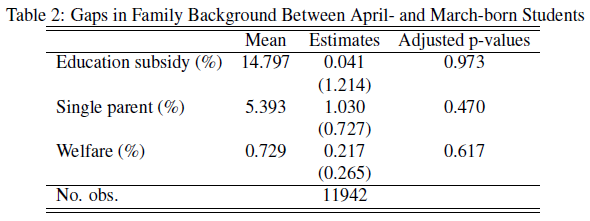
\includegraphics[scale = 1]{0904tanji/T2}
    \end{figure}

    \begin{itemize}
      \item Overall, the differences in parental characteristics and birth outcomes by birth month are small, if any.
      \item Limited ability to time the birth: given that the average child-bearing age is high, postponing conception can lower the chance of pregnancy.
    \end{itemize}
    \section{Data}


    \subsection{Overview}

    \paragraph{Standardized achievement tests and questionnaires to measure noncognitive skills}

    \begin{itemize}
      \item Administered data in an anonymous province in a suburb of Tokyo every April since 2015 (fourth through ninth grade students).
      \item Almost all the students take the exam (One municipality opt out to take the skill assesment).
      \item 708 elementary and 356 junior high schools in 62 municipalities are included.
    \end{itemize}

    \begin{figure}[ht]
      \centering
      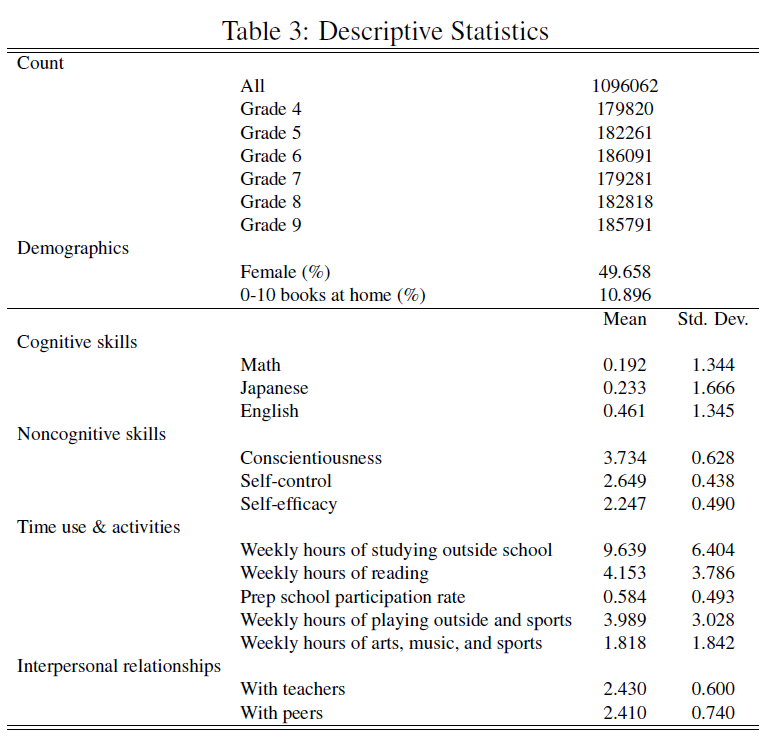
\includegraphics[scale = 1]{0904tanji/T3}
    \end{figure}

    \subparagraph{Descriptive Statistics}

    \begin{itemize}
      \item 1.1 million student-year observations.
      \item Attrition rates in each year to the next are about 2\%, and 8\% at sixth to seventh grade.
      \item Those who enter selective private junior high school have higher cognitive and noncognitive skills, but does not prevent comparison across grades.
      \item Proxy for SES: the number of books.
    \end{itemize}

    \subsection{Variable Definitions}

    \paragraph{Cognitive Skills}

    \begin{itemize}
      \item Math and Japanese tests for all grades and English for eighth and ninth.
      \item Tests are designed to enable comparisons of scores across different grades and test dates (item response theory).
      \item Scores are normalized using the mean and s.d. of a certain graders.
    \end{itemize}

    \paragraph{Noncognitive Skills}

    \begin{itemize}
      \item In a 40-minute questionnaire to collect information on students' noncognitive skills: conscientiousness, self-control, and self-efficacy.
      \item Each cohort answered questions to measure only one of the three skills (Figure 2).
    \end{itemize}

    \begin{figure}[ht]
      \centering
      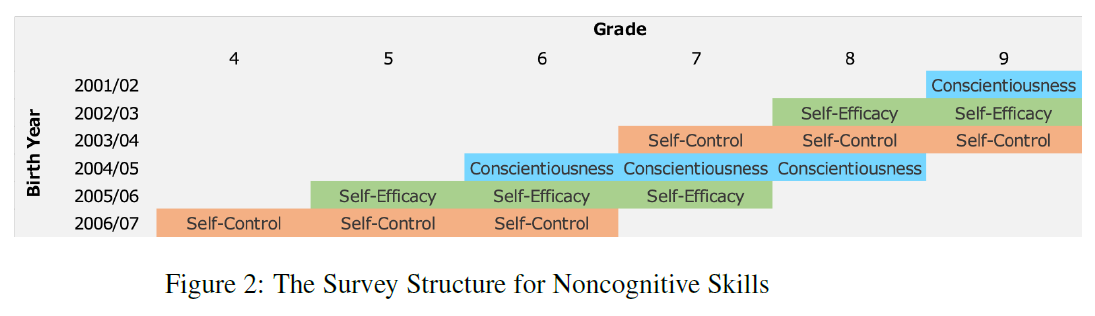
\includegraphics[scale = .8]{0904tanji/F2}
    \end{figure}

    \paragraph{Human Capital Investment and Interpersonal}

    \begin{itemize}
      \item Questionnaire about students' time use, prep school participation, and quality of relationships with teachers and peers
      \begin{itemize}
        \item as direct measures of human capital.
        \item can influence a student's behavior and skills.
      \end{itemize}
      \item Time use of reading, playing outside and sports, and organized out-of-school activities (sports, music, and arts).
      \begin{itemize}
        \item The original response is provided as as interval: taking midpoint. If students responded that they study 21 hrs or more per week, assume 21 $\times 1.25$.
      \end{itemize}
      \item Prep school attendance
      \begin{itemize}
        \item Average annual expenditure on prep schools: 218,000 for public elementary school students, and 301,200 for public junior high school students.
      \end{itemize}
      \item Quality of relationships with teachers (four-point scale).
      \begin{itemize}
        \item 'Did your teacher(s) assist you adequately?'
        \item 'Did your teacher(s) recognize your strengths?'
        \item 'Did your teacher(s) help you understand content in class that you found confusing?'
      \end{itemize}
      \item Quality of relationships with frends (four-point scale)
      \begin{itemize}
        \item 'Did your friend(s) recognize your strengths?'
      \end{itemize}
    \end{itemize}


    \section{Month-of-Birth Effects on Skills and High School Quality}

    \subsection{Cognitive Skills}

    \begin{itemize}
      \item Two important features(Figre 3)
      \begin{itemize}
        \item Average test scores increase with age at a decreasing rate.
        \item Mean test scores ris discontinuously at the grade cutoff for some grades.
      \end{itemize}
      \item Regresion (Table 4): p-values are adjusted by a method that controls for a false discovery rate (Benjamini and Hochberg, 1995)
      \begin{itemize}
        \item The gap between the oldest and the youngest students in a given grade is .350 standard deviations for grade four; .125 s.d. for grade ninth (statistically significant from that of grade four).
        \item Excluding March- and April-born students does not change the results.
      \end{itemize}
    \end{itemize}

    \begin{figure}[ht]
      \centering
      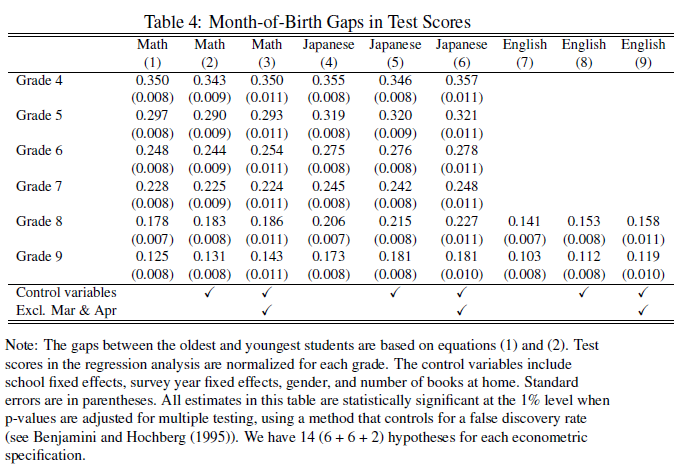
\includegraphics[scale = 1.2]{0904tanji/T4}
    \end{figure}

    \subsection{Noncognitive Skills}No gaps are driven by the questions themselves (identical questions across different grades and survey years).

    \begin{itemize}
      \item Noncognitive skills tend to be decrease with grade.
      \begin{itemize}
        \item Soto et al. (2011), Robins et al.(2002), Denissen et al. (2013)
        \item As childrens grow, their parents and teachers increasingly expect responsible behavior, while children internalize new values and develop a behavioral repertoire to accomodate them.
      \end{itemize}
      \item Older students within the same grade have better noncognitive skills.
      \item Regression (Table 5)
      \begin{itemize}
        \item The estimated gaps are .098 standard deviations in conscientiousness at grade six. The size of the gaps are nearly constant across grades.
        \item The effect size is smaller than that for cognitive skills.
        \item The month-of-birth effect is constant across grades, unlike that on cognitive skills.
      \end{itemize}
    \end{itemize}

    \begin{figure}[ht]
      \centering
      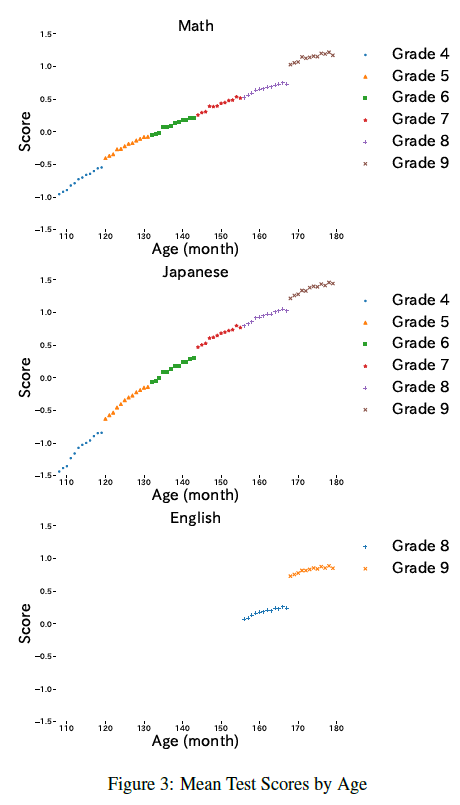
\includegraphics[scale = 1]{0904tanji/F3}
      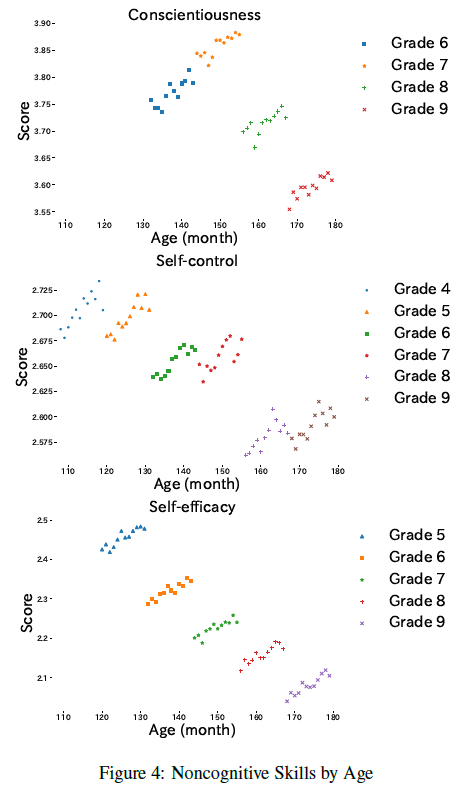
\includegraphics[scale = 1]{0904tanji/F4}
    \end{figure}

    \section{Month-of-Birth Effects on Human Capital Investment and Interpersonal Relationships}

    \begin{itemize}
      \item The average weekly hours of study outside of school.
      \begin{itemize}
        \item increase with grade, but younger students in a given grade study longer hours: .295 hours among ninth graders.
        \item weekly hours of reading and enrollment rate for a prep school show the similar tendencies.
      \end{itemize}
      \item The average hours per week outside school.
      \begin{itemize}
        \item Younger students in a given grade play sports for fewer hours than older students in any grade: .517 hours at most.
        \item (We cannot disentangle hours for sports from those for art and music activities.)
        \item Students shift to prep school.
      \end{itemize}
    \end{itemize}

    \begin{figure}[ht]
      \centering
      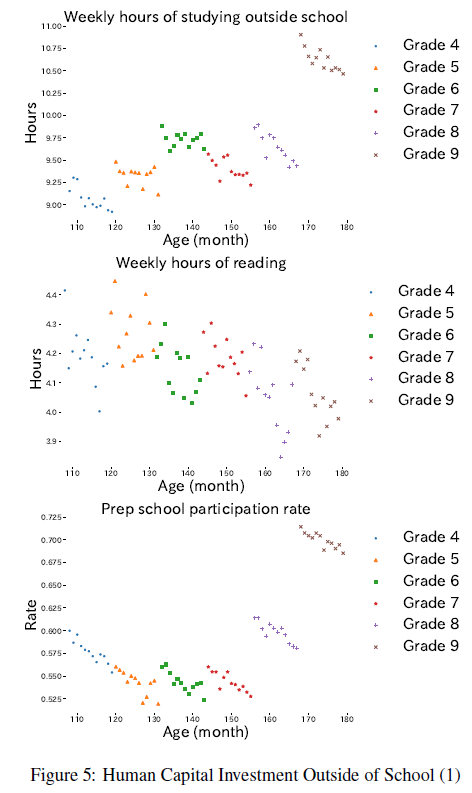
\includegraphics[scale = 1]{0904tanji/F5}
      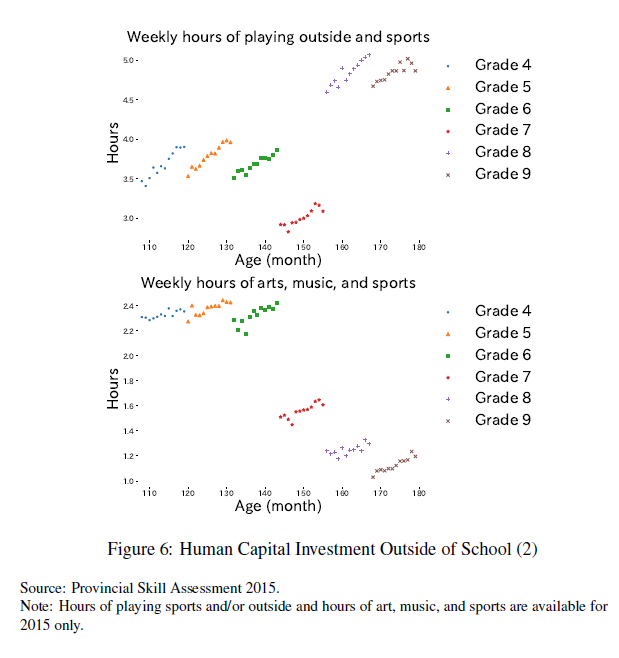
\includegraphics[scale = 1]{0904tanji/F6}
    \end{figure}

    \subsection{Interpersonal Relationships}

    \begin{itemize}
      \item Self-assessed relationships with teachers and peers.
      \begin{itemize}
        \item Older students have better relationships with teachers and peers: .052-.089 s.d. poorer relationships with teachers and .096-.127 s.d. with peers.
      \end{itemize}
    \end{itemize}

    \begin{figure}[ht]
      \centering
      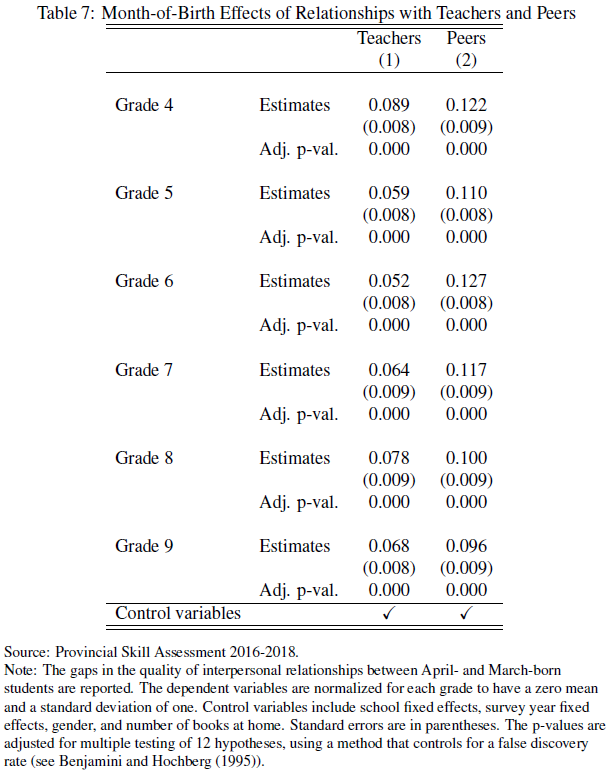
\includegraphics[scale = 1.1]{0904tanji/T7}
    \end{figure}

    \begin{figure}[ht]
      \centering
      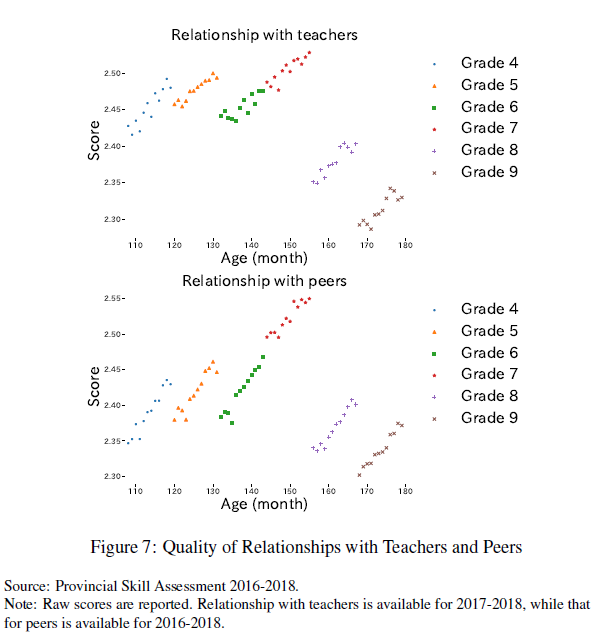
\includegraphics[scale = 1]{0904tanji/F7}
      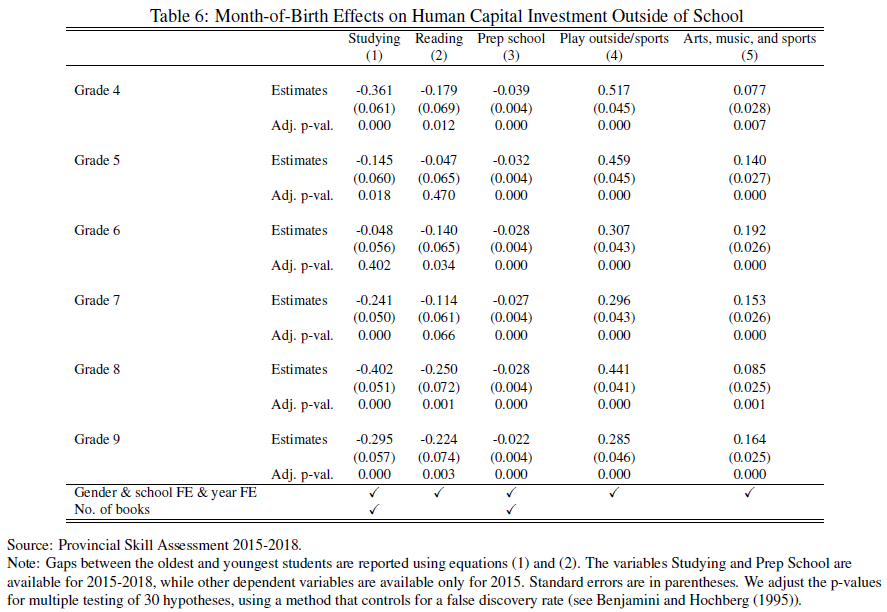
\includegraphics[scale = 1]{0904tanji/T6}
    \end{figure}

    \section{Discussion}

    \paragraph{Cognitive Skills}

    \begin{itemize}
      \item The most comparable study to the current paper is Bedard and Dhuey (2006): TIMSS
      \item The size of the effect is relatively modest (0.25-0.31 standard deviations for grade four and 0.23 standard deviations for grade eight among Japanese students).
    \end{itemize}

    \paragraph{Noncognitive Skills}

    \begin{itemize}
      \item Month-of-birth effects on noncognitive skills remain constant from grade four to nine.
      \begin{itemize}
        \item Only a few previous papers have estimated month-of-birth effects on noncognitive skills: Datar and Gottfried (2015) and Peña and Duckworth (2018)
        \item Data that cover a broader range of noncognitive skills for a longer period of time than in previous studies.
      \end{itemize}
    \end{itemize}

    \paragraph{human capital investment and interpersonal relationships}

    \begin{itemize}
      \item the youngest students study and read more hours and are more likely to attend a prep school than are the oldest students in the same grade.
      \begin{itemize}
        \item Hours of studying improve the GPA of first year students at a US college (Stinebrickner and Stinebrickner, 2008)
        \item After-school education programs improve Japanese students’ test scores. (Akabayashi et al., 2018)
      \end{itemize}
      \item Low participation at sports, music, and art activities and poor-quality relationships with peers and teachers may lead to disadvantage in noncognitive skills development.
      \begin{itemize}
        \item Ishihara et al. (2018): strong association between sports experience and noncognitive skills.
        \item Moreno et al. (2011): music training enhances noncognitive skills.
        \item Wu et al. (2018): strong association between teacher-child relation and children’s social skills.
      \end{itemize}
    \end{itemize}

    \paragraph{Efficiency}

    \begin{itemize}
      \item Compensatory skill investment is an individually optimal strategy in the short run, but may be suboptimal from a long-term and/or societal perspective.
      \begin{itemize}
        \item the same argument applies to older students because they may underinvest in cognitive skills.
        \item Kinsler and Pavan (forthcoming)
      \end{itemize}
      \item The youngest students suffer poor relationships with teachers and peers
      \begin{itemize}
        \item Even if part of the month-of-birth gaps disappear by adulthood, month of birth hurts the welfare of younger children in a given grade cohort.
        \item Matsubayashi and Ueda (2015): month of birth affects the suicide rate among young Japanese aged 15-25 years.
        \item Kawaguchi (2008): noncognitive skill gaps may be one of key driving forces behind the month-of-birth effects on earnings at age 30-34 years
        \item If month-of-birth effects on noncognitive skills remain in adulthood, they are likely to translate into an earnings gap.
      \end{itemize}
    \end{itemize}

    \section{Coclusion}

    \begin{itemize}
      \item Their findings also have implications for the current policy debate regarding whether to change the school starting date in Japan from April to September.
      \item One of the possible consequences is an increase in cohort size, because children born between April 2014 and August 2015 would start school together.

      \item Limitations:
      \begin{enumerate}
        \item Their data do not include skills and other outcomes in adulthood.
        \item They cannot identify causal effects of time use and interpersonal relationships on skils.
      \end{enumerate}
    \end{itemize}


    %\begin{figure}[]
    %    \centering
    %    \includegraphics[scale = 1]{0904tanji/}
    %\end{figure}

    \biblio

\end{document}
